\chapter{VaR and Credit Risk}\label{var-and-credit-risk}

VaR is an acronym of ‘Value at Risk’, and is a tool which is used by many firms and banks to establish the level of financial risk within its firm. The VaR is calculated for an investments of a company’s investments or perhaps for checking the riks levels of a portfolio managed by the wealth management branch of a bank or a boutique firm.

\section{Value at Risk}\label{value-at-risk}

The value at risk (VaR) of a portfolio is a function of two parameters
(time horizon and confidence level) and it is usually involved when it
is important to know to a certain confidence level how
much will be the maximum loss in the next $N$ days. 

It can be interpreted as the loss level over \(N\) days that has a 
probability of only \((100 - X)\%\) of being exceeded.
Mathematically the VaR is the loss corresponding to the
\((100-X)\textrm{th}\) percentile of the distribution of the change in
the value of the portfolio over the next \(N\) days. 

For example, with \(N=1\) and \(X=95\), VaR is the fifth percentile of the distribution of
changes in the value of the portfolio over the next day (e.g. in Figure~\ref{fig:var_loss}
the graphical representation of the VaR assuming a normal
distribution for the changes of value.

\begin{figure}
\centering
  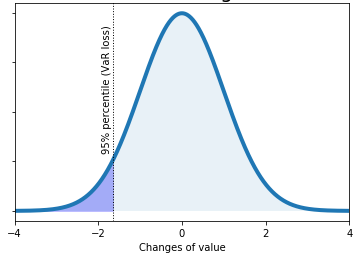
\includegraphics[width=0.6\linewidth]{figures/lecture_9_2_0.png}
  \caption{Example of 95\% VaR on the distribution of changes in the value.}
  \label{fig:var_loss}
\end{figure}
    
VaR is useful to summarize all the information about the risk of a
portfolio in one single number, but this can also be considered its main
limitation (as it implies too much simplification).

Concerning the time horizon parameter it is usually set to \(N=1\) since
it is not easy to estimate market variables over periods longer than one
day. To generalize the VaR estimate it is assumed:

\begin{equation}
\textrm{N-day VaR} = \textrm{1-day VaR}\times \sqrt{N}
\label{eq:var_horizon}
\end{equation}

This relation is true only if the changes of value of the portfolio over
the considered period of time have independent and identical normal
distributions with mean 0 (otherwise it is just an approximation).

\section{How to Estimate the VaR}\label{how-to-estimate-the-var}

Three are the methods that can be used to estimate the VaR.
In this Section they will be reviewed.

In the proposed examples historical series of Apple and Netflix will 
are used. Data is saved in \href{}{historical\_data.csv}.
It can be inspected as usual with \texttt{pandas}.
We will assume to have a portfolio made of 60\% of AAPL and 40\% NFLX stocks.

\begin{tcolorbox}[breakable, size=fbox, boxrule=1pt, pad at break*=1mm,colback=cellbackground, colframe=cellborder]
\begin{Verbatim}[commandchars=\\\{\}]
\PY{k+kn}{import} \PY{n+nn}{pandas} \PY{k}{as} \PY{n+nn}{pd}
\PY{k+kn}{import} \PY{n+nn}{numpy} \PY{k}{as} \PY{n+nn}{np}

\PY{n}{w} \PY{o}{=} \PY{n}{np}\PY{o}{.}\PY{n}{array}\PY{p}{(}\PY{p}{[}\PY{l+m+mf}{0.6}\PY{p}{,} \PY{l+m+mf}{0.4}\PY{p}{]}\PY{p}{)}
\PY{n}{df} \PY{o}{=} \PY{n}{pd}\PY{o}{.}\PY{n}{read\PYZus{}csv}\PY{p}{(}\PY{l+s+s2}{\PYZdq{}}\PY{l+s+s2}{quandl.csv}\PY{l+s+s2}{\PYZdq{}}\PY{p}{)}
\PY{n}{aapl} \PY{o}{=} \PY{n}{df}\PY{p}{[}\PY{n}{df}\PY{p}{[}\PY{l+s+s1}{\PYZsq{}}\PY{l+s+s1}{ticker}\PY{l+s+s1}{\PYZsq{}}\PY{p}{]}\PY{o}{==}\PY{l+s+s2}{\PYZdq{}}\PY{l+s+s2}{AAPL}\PY{l+s+s2}{\PYZdq{}}\PY{p}{]}\PY{o}{.}\PY{n}{copy}\PY{p}{(}\PY{p}{)}
\PY{n}{nlfx} \PY{o}{=} \PY{n}{df}\PY{p}{[}\PY{n}{df}\PY{p}{[}\PY{l+s+s1}{\PYZsq{}}\PY{l+s+s1}{ticker}\PY{l+s+s1}{\PYZsq{}}\PY{p}{]}\PY{o}{==}\PY{l+s+s2}{\PYZdq{}}\PY{l+s+s2}{NFLX}\PY{l+s+s2}{\PYZdq{}}\PY{p}{]}\PY{o}{.}\PY{n}{copy}\PY{p}{(}\PY{p}{)}
		
\PY{n}{aapl}\PY{p}{[}\PY{l+s+s1}{\PYZsq{}}\PY{l+s+s1}{rets}\PY{l+s+s1}{\PYZsq{}}\PY{p}{]} \PY{o}{=} \PY{n}{aapl}\PY{p}{[}\PY{l+s+s1}{\PYZsq{}}\PY{l+s+s1}{adj\PYZus{}close}\PY{l+s+s1}{\PYZsq{}}\PY{p}{]}\PY{o}{/}\PY{n}{aapl}\PY{p}{[}\PY{l+s+s1}{\PYZsq{}}\PY{l+s+s1}{adj\PYZus{}close}\PY{l+s+s1}{\PYZsq{}}\PY{p}{]}\PY{o}{.}\PY{n}{shift}\PY{p}{(}\PY{l+m+mi}{1}\PY{p}{)} \PY{o}{\PYZhy{}} \PY{l+m+mi}{1}
\PY{n}{nflx}\PY{p}{[}\PY{l+s+s1}{\PYZsq{}}\PY{l+s+s1}{rets}\PY{l+s+s1}{\PYZsq{}}\PY{p}{]} \PY{o}{=} \PY{n}{nflx}\PY{p}{[}\PY{l+s+s1}{\PYZsq{}}\PY{l+s+s1}{adj\PYZus{}close}\PY{l+s+s1}{\PYZsq{}}\PY{p}{]}\PY{o}{/}\PY{n}{nflx}\PY{p}{[}\PY{l+s+s1}{\PYZsq{}}\PY{l+s+s1}{adj\PYZus{}close}\PY{l+s+s1}{\PYZsq{}}\PY{p}{]}\PY{o}{.}\PY{n}{shift}\PY{p}{(}\PY{l+m+mi}{1}\PY{p}{)} \PY{o}{\PYZhy{}} \PY{l+m+mi}{1}

\PY{n+nb}{print} \PY{p}{(}\PY{n}{aapl}\PY{o}{.}\PY{n}{head}\PY{p}{(}\PY{p}{)}\PY{p}{)}

            date ticker adj\_close      rets
4201  2018-03-27   AAPL    168.340       NaN
4202  2018-03-26   AAPL    172.770  0.026316
4203  2018-03-23   AAPL    164.940 -0.045320
4204  2018-03-22   AAPL    168.845  0.023675
4205  2018-03-21   AAPL    171.270  0.014362
\end{Verbatim}
\end{tcolorbox}

\subsection{Historical Simulation}\label{historical-simulation}

In order to estimate the VaR from an historical series, we need to
collect the market variables affecting the portfolio over the last \(N\)
days (with \(N\) quite large).

The variation over each day in our time interval will provide different
scenarios to be applied to today's market simulation so that for each of
them we need to compute the variation in the portfolio value
(\(\Delta P\)). 

Given the distribution of the simulated scenarios the VaR estimate 
will be its (100 - X)\% percentile. 

Of course such historical simulation relies on the assumption that past
behaviors are indicative of what might happen in the future, that's why it 
is important that out historical series was as large as possible.

As an example imagine a portfolio \(P\) whose value depends only on two market
variables (\(x_1(t) , x_2(t)\)). From the historical series of these
variables we can determine various \emph{simulated} portfolio
values:

\[P_i(t_n+1) = P\Big(x_1(t_n)\cfrac{(x_1(t_i)-x_1(t_{i-1}))}{x_1(t_{i-1})}, x_2(t_n)\cfrac{(x_2(t_i)-x_2(t_{i-1}))}{x_2(t_{i-1})}\Big)\]

Essentially re-scaling the market variables according to the variation
between day \(i\) and \(i-1\) we can draw a distribution of the possible
changes in the portfolio value \(P_i\) and then compute the VaR taking
the appropriate percentile.

Using the historical series seen above the procedure can be outlined as follows. Figure~\ref{fig:hist_var} shows the resulting VaR.

\begin{tcolorbox}[breakable, size=fbox, boxrule=1pt, pad at break*=1mm,colback=cellbackground, colframe=cellborder]
\begin{Verbatim}[commandchars=\\\{\}]
\PY{c+c1}{\PYZsh{} historical VaR}
\PY{k+kn}{import} \PY{n+nn}{numpy} \PY{k}{as} \PY{n+nn}{np}
				
\PY{n}{rets} \PY{o}{=} \PY{p}{[}\PY{p}{]}
\PY{k}{for} \PY{n}{i} \PY{o+ow}{in} \PY{n+nb}{range}\PY{p}{(}\PY{l+m+mi}{1}\PY{p}{,} \PY{n+nb}{len}\PY{p}{(}\PY{n}{aapl}\PY{p}{)}\PY{p}{)}\PY{p}{:}
    \PY{n}{rets}\PY{o}{.}\PY{n}{append}\PY{p}{(}\PY{n}{w}\PY{p}{[}\PY{l+m+mi}{0}\PY{p}{]}\PY{o}{*}\PY{n}{aapl}\PY{o}{.}\PY{n}{iloc}\PY{p}{[}\PY{n}{i}\PY{p}{]}\PY{p}{[}\PY{l+s+s1}{\PYZsq{}}\PY{l+s+s1}{rets}\PY{l+s+s1}{\PYZsq{}}\PY{p}{]} \PY{o}{+} \PY{n}{w}\PY{p}{[}\PY{l+m+mi}{1}\PY{p}{]}\PY{o}{*}\PY{n}{nflx}\PY{o}{.}\PY{n}{loc}\PY{p}{[}\PY{n}{i}\PY{p}{]}\PY{p}{[}\PY{l+s+s1}{\PYZsq{}}\PY{l+s+s1}{rets}\PY{l+s+s1}{\PYZsq{}}\PY{p}{]}\PY{p}{)}
		
\PY{n}{price} \PY{o}{=} \PY{p}{[}\PY{n}{aapl}\PY{o}{.}\PY{n}{iloc}\PY{p}{[}\PY{o}{\PYZhy{}}\PY{l+m+mi}{1}\PY{p}{]}\PY{p}{[}\PY{l+s+s1}{\PYZsq{}}\PY{l+s+s1}{adj\PYZus{}close}\PY{l+s+s1}{\PYZsq{}}\PY{p}{]}\PY{p}{,} \PY{n}{nflx}\PY{o}{.}\PY{n}{iloc}\PY{p}{[}\PY{o}{\PYZhy{}}\PY{l+m+mi}{1}\PY{p}{]}\PY{p}{[}\PY{l+s+s1}{\PYZsq{}}\PY{l+s+s1}{adj\PYZus{}close}\PY{l+s+s1}{\PYZsq{}}\PY{p}{]}\PY{p}{]}
		
\PY{n}{portfolio\PYZus{}price} \PY{o}{=} \PY{n}{w}\PY{o}{.}\PY{n}{dot}\PY{p}{(}\PY{n}{price}\PY{p}{)}
		
\PY{n}{hist\PYZus{}var} \PY{o}{=} \PY{n}{portfolio\PYZus{}price}\PY{o}{*}\PY{n}{np}\PY{o}{.}\PY{n}{percentile}\PY{p}{(}\PY{n}{rets}\PY{p}{,} \PY{l+m+mi}{1}\PY{p}{)}
\PY{n+nb}{print} \PY{p}{(}\PY{l+s+s1}{\PYZsq{}}\PY{l+s+s1}{Historical VAR is }\PY{l+s+si}{\PYZob{}:.3f\PYZcb{}}\PY{l+s+s1}{\PYZsq{}}\PY{o}{.}\PY{n}{format}\PY{p}{(}\PY{n}{hist\PYZus{}var}\PY{p}{)}\PY{p}{)}

Historical VAR is -2.412
\end{Verbatim}
\end{tcolorbox}

\begin{figure}
	\centering
	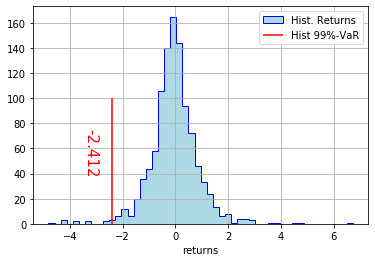
\includegraphics[width=0.7\textwidth]{figures/Untitled_0_1.png}
	\caption{Distribution of the changes of values estimated from historical data. The red line shows the 99\% VaR.}
	\label{fig:hist_var}
\end{figure}

\subsection{Model Approach}\label{model-approach}

Our portfolio \(P\) consists of different amounts \(w_i\)
invested on two assets. If with \(\Delta x_i\) we denote the daily
return of the $i$th asset the change in the value of the portfolio can be
expressed as:

\[\Delta P = \sum_{i=1}^n w_i \Delta x_i\]

If we then assume that the asset variations are normally distributed
with mean 0 (in this approach is typical to assume the expected change
in a market variable over the considered period zero), \(\Delta P\) will
be normally distributed (as a sum of normal distribution) with zero
mean.

To estimate the VaR we just need to compute the standard deviation of
\(\Delta P\). In the general case with many different assets we define
\(\sigma_i\) the daily volatility of the $i$th asset and with
\(\rho_{ij}\) the correlation coefficient between the assets $i$ and $j$.
The variance of \(\Delta P\) can then be expressed as:

\begin{align*}\sigma^2_P & = \sum_{i=1}^{n}\sum_{j=1}^{n}\rho_{ij}w_i w_j \sigma_i \sigma_j \\
& = \sum_{i=1}^{n} w_i^2 \sigma_i^2 + 2 \sum_{i=1}^{n}\sum_{j<i}^{n}\rho_{ij}w_i w_j \sigma_i \sigma_j 
\end{align*}

As in the previous case if we are interested in a longer time horizon we
can use Eq.~\ref{eq:var_horizon}.

Once we have the variance of \(\Delta P\) it is easy to determine the appropriate percentile using the equations described in Appendix~\ref{transformation-to-standard-normal}.


\subsection{Monte Carlo Simulation}\label{monte-carlo-simulation}

A very useful alternative to the previous approaches is using a Monte
Carlo simulation to generate the probability distribution for the
\(\Delta P\) distribution. 

Imagine we need to compute the 1-day VaR for our example portfolio
the simulation can be done either generating random returns from a distribution with mean and standard deviation obtained from the historical data of each stock, or by simulating the evolution 
of all the portfolio market variables in one day.

Let's start from the first case, computing mean and standard deviation of each historical data-set. We will then throw various simulated returns from a multivariate Gaussian with such means and variances. 
One useful aspect of this method is that in principal other distribution could be used instead of a Gaussian.
Once we have the distribution of returns the VaR can be computed as usual, the example distribution is shown in Fig.~\ref{fig:mc1_var}.

\begin{tcolorbox}[breakable, size=fbox, boxrule=1pt, pad at break*=1mm,colback=cellbackground, colframe=cellborder]
\begin{Verbatim}[commandchars=\\\{\}]
\PY{c+c1}{\PYZsh{} MC simulated VaR 1}
\PY{k+kn}{from} \PY{n+nn}{scipy}\PY{n+nn}{.}\PY{n+nn}{stats} \PY{k}{import} \PY{n}{norm}		
\PY{k+kn}{from} \PY{n+nn}{scipy}\PY{n+nn}{.}\PY{n+nn}{stats} \PY{k}{import} \PY{n}{multivariate\PYZus{}normal}
		
\PY{n}{mean} \PY{o}{=} \PY{p}{[}\PY{n}{np}\PY{o}{.}\PY{n}{mean}\PY{p}{(}\PY{n}{aapl}\PY{p}{[}\PY{l+s+s1}{\PYZsq{}}\PY{l+s+s1}{rets}\PY{l+s+s1}{\PYZsq{}}\PY{p}{]}\PY{p}{)}\PY{p}{,} \PY{n}{np}\PY{o}{.}\PY{n}{mean}\PY{p}{(}\PY{n}{nflx}\PY{p}{[}\PY{l+s+s1}{\PYZsq{}}\PY{l+s+s1}{rets}\PY{l+s+s1}{\PYZsq{}}\PY{p}{]}\PY{p}{)}\PY{p}{]}
\PY{n}{std} \PY{o}{=} \PY{p}{[}\PY{n}{np}\PY{o}{.}\PY{n}{std}\PY{p}{(}\PY{n}{aapl}\PY{p}{[}\PY{l+s+s1}{\PYZsq{}}\PY{l+s+s1}{rets}\PY{l+s+s1}{\PYZsq{}}\PY{p}{]}\PY{p}{)}\PY{p}{,} \PY{n}{np}\PY{o}{.}\PY{n}{std}\PY{p}{(}\PY{n}{nflx}\PY{p}{[}\PY{l+s+s1}{\PYZsq{}}\PY{l+s+s1}{rets}\PY{l+s+s1}{\PYZsq{}}\PY{p}{]}\PY{p}{)}\PY{p}{]}
		
\PY{n}{mvnorm} \PY{o}{=} \PY{n}{multivariate\PYZus{}normal}\PY{p}{(}\PY{n}{mean}\PY{o}{=}\PY{n}{mean}\PY{p}{,} \PY{n}{cov}\PY{o}{=}\PY{p}{[}\PY{p}{[}\PY{n}{std}\PY{p}{[}\PY{l+m+mi}{0}\PY{p}{]}\PY{o}{*}\PY{o}{*}\PY{l+m+mi}{2}\PY{p}{,} \PY{l+m+mi}{0}\PY{p}{]}\PY{p}{,}
                                             \PY{p}{[}\PY{l+m+mi}{0}\PY{p}{,} \PY{n}{std}\PY{p}{[}\PY{l+m+mi}{1}\PY{p}{]}\PY{o}{*}\PY{o}{*}\PY{l+m+mi}{2}\PY{p}{]}\PY{p}{]}\PY{p}{)}
\PY{n}{n\PYZus{}sims} \PY{o}{=} \PY{l+m+mi}{100000}
\PY{n}{sim\PYZus{}returns} \PY{o}{=} \PY{n}{mvnorm}\PY{o}{.}\PY{n}{rvs}\PY{p}{(}\PY{n}{n\PYZus{}sims}\PY{p}{)}
\PY{n}{p\PYZus{}returns} \PY{o}{=} \PY{p}{[}\PY{n}{w}\PY{o}{.}\PY{n}{dot}\PY{p}{(}\PY{n}{s}\PY{p}{)} \PY{k}{for} \PY{n}{s} \PY{o+ow}{in} \PY{n}{sim\PYZus{}returns}\PY{p}{]}
\PY{n}{mc\PYZus{}var} \PY{o}{=} \PY{n}{portfolio\PYZus{}price} \PY{o}{*} \PY{n}{np}\PY{o}{.}\PY{n}{percentile}\PY{p}{(}\PY{n}{p\PYZus{}returns}\PY{p}{,} \PY{l+m+mi}{1}\PY{p}{)}
\PY{n+nb}{print}\PY{p}{(}\PY{l+s+s1}{\PYZsq{}}\PY{l+s+s1}{Simulated VAR is }\PY{l+s+si}{\PYZob{}\PYZcb{}}\PY{l+s+s1}{\PYZsq{}}\PY{p}{,} \PY{n}{mc\PYZus{}var}\PY{p}{)}

Simulated VAR is \{\} -2.114679008811982
\end{Verbatim}
\end{tcolorbox}

\begin{figure}[htb]
	\centering
	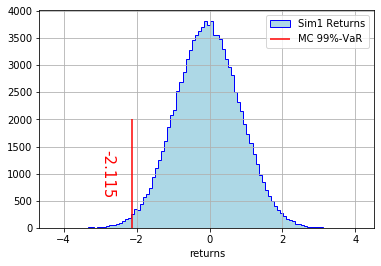
\includegraphics[width=0.7\textwidth]{figures/Untitled_2_1.png}
	\caption{Distribution of the changes of values estimated from simulated data. The red line shows the 99\% VaR.}
	\label{fig:mc1_var}
\end{figure}

This result can be compared with the VaR estimated with a simulation of the daily evolution of the stock price. We will use the log-normal evolution described in Section~\ref{derivation-of-log-normal-stochastic-differential-equation} where $\mu$ and $\sigma@$ are the mean and variance estimated from the historical series. Figure~\ref{fig:mc2_var} shows the resulting distribution of the returns.

\begin{tcolorbox}[breakable, size=fbox, boxrule=1pt, pad at break*=1mm,colback=cellbackground, colframe=cellborder]
\begin{Verbatim}[commandchars=\\\{\}]
\PY{k+kn}{from} \PY{n+nn}{numpy} \PY{k}{import} \PY{n}{exp}\PY{p}{,} \PY{n}{sqrt}
		
\PY{n}{T} \PY{o}{=} \PY{l+m+mi}{1}
\PY{n}{trials} \PY{o}{=} \PY{l+m+mi}{100000}
\PY{n}{dP} \PY{o}{=} \PY{p}{[}\PY{p}{]}
		
\PY{k}{for} \PY{n}{\PYZus{}} \PY{o+ow}{in} \PY{n+nb}{range}\PY{p}{(}\PY{n}{trials}\PY{p}{)}\PY{p}{:}
    \PY{n}{s} \PY{o}{=} \PY{l+m+mi}{0}
    \PY{k}{for} \PY{n}{i} \PY{o+ow}{in} \PY{n+nb}{range}\PY{p}{(}\PY{l+m+mi}{2}\PY{p}{)}\PY{p}{:}
        \PY{n}{s} \PY{o}{+}\PY{o}{=} \PY{n}{w}\PY{p}{[}\PY{n}{i}\PY{p}{]} \PY{o}{*} \PY{n}{price}\PY{p}{[}\PY{n}{i}\PY{p}{]} \PY{o}{*} \PY{n}{exp}\PY{p}{(}\PY{p}{(}\PY{n}{mean}\PY{p}{[}\PY{n}{i}\PY{p}{]} \PY{o}{\PYZhy{}} \PY{l+m+mf}{0.5} \PY{o}{*} \PY{n}{std}\PY{p}{[}\PY{n}{i}\PY{p}{]}\PY{o}{*}\PY{o}{*}\PY{l+m+mi}{2}\PY{p}{)} \PY{o}{*} \PY{n}{T} \PY{o}{+} 
                                   \PY{n}{std}\PY{p}{[}\PY{n}{i}\PY{p}{]} \PY{o}{*} \PY{n}{sqrt}\PY{p}{(}\PY{n}{T}\PY{p}{)} \PY{o}{*} \PY{n}{normal}\PY{p}{(}\PY{p}{)}\PY{p}{)}
    \PY{n}{dP}\PY{o}{.}\PY{n}{append}\PY{p}{(}\PY{n}{portfolio\PYZus{}price} \PY{o}{\PYZhy{}} \PY{n}{s}\PY{p}{)}
		
\PY{n}{mc\PYZus{}var2} \PY{o}{=} \PY{n}{np}\PY{o}{.}\PY{n}{percentile}\PY{p}{(}\PY{n}{dP}\PY{p}{,} \PY{l+m+mi}{1}\PY{p}{)}
\PY{n+nb}{print}\PY{p}{(}\PY{l+s+s1}{\PYZsq{}}\PY{l+s+s1}{Simulated VAR is }\PY{l+s+si}{\PYZob{}\PYZcb{}}\PY{l+s+s1}{\PYZsq{}}\PY{p}{,} \PY{n}{mc\PYZus{}var2}\PY{p}{)}

Simulated VAR is \{\} -1.9213098361249987
\end{Verbatim}
\end{tcolorbox}

\begin{figure}[htb]
	\centering
	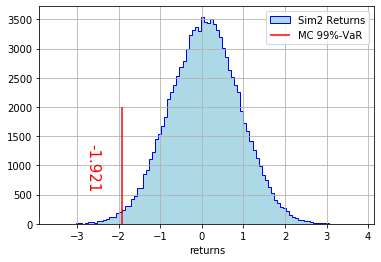
\includegraphics[width=0.7\textwidth]{figures/Untitled_3_1.png}
	\caption{Distribution of the changes of values estimated from simulation of the evolution of the stock prices. The red line shows the 99\% VaR.}
	\label{fig:mc2_var}
\end{figure}


\subsection{Stress and Back Testing}\label{stress-testing-and-back-testing}

In addition to calculating the value at risk of a portfolio, it could be useful to 
check how it would behave under the most extreme moves seen in the last years.

This kind of test is called \emph{stress test} and it is done by extracting from the historical series, particular days with exceptional large variation of our market variables, im order to check
how the portfolio moves.
 
The idea is to take into account extreme events that can more frequently in reality 
than in a simulation where Gaussian tails are assumed hence are quite hard to simulate
(e.g. a 5-standard deviation move should happen once every 7000 years
but in practice can be observed twice over 10 years).

How can we compute how likely is a $n\sigma$ event (assuming Gaussian distribution) ?
The probability of such a daily event is given by 1 over the total probability of having an 
event with a probability of $\pm n\sigma$ or more (the 252 factor comes to the number of working days per year).

\begin{tcolorbox}[breakable, size=fbox, boxrule=1pt, pad at break*=1mm,colback=cellbackground, colframe=cellborder]
\begin{Verbatim}[commandchars=\\\{\}]
\PY{k+kn}{from} \PY{n+nn}{scipy}\PY{n+nn}{.}\PY{n+nn}{stats} \PY{k}{import} \PY{n}{norm}

\PY{n}{prob} \PY{o}{=} \PY{n}{norm}\PY{o}{.}\PY{n}{cdf}\PY{p}{(}\PY{o}{\PYZhy{}}\PY{l+m+mi}{5}\PY{p}{)} \PY{o}{*} \PY{l+m+mi}{2} \PY{c+c1}{\PYZsh{} e.g. consider +\PYZhy{} 5sigma movements}
\PY{n}{nyears} \PY{o}{=} \PY{l+m+mi}{1}\PY{o}{/}\PY{n}{prob}\PY{o}{/}\PY{l+m+mi}{252}
\PY{n+nb}{print} \PY{p}{(}\PY{n}{nyears}\PY{p}{)}

6921.737673091067
    \end{Verbatim}
\end{tcolorbox}

Another important check that could be done is the so-called \emph{back testing}
which consists of checking how well the VaR estimate would have
performed in the past. Basically it has to be tested how often the daily
loss exceeded the N-days X\% VaR just computed. If it happens on about
(100-X)\% of the times we can be confident that our estimate is correct.

\section{Credit-VaR (Cr-VaR)}\label{credit-var-cr-var}

The Credit-VaR is a measure of the default risk associated to one or
multiple counterparties in a specific portfolio, and it is defined on
the overall exposure to all the counterparties involved. Cr-VaR is
defined in the usual way Value at Risk measures are defined (i.e. as
percentile of a loss). Our exposure Ex at the default date is defined
as:

\[ \textrm{Ex} = (\sum \Pi(\tau, T))^{+}\]

where \(\Pi(\tau,T)\) represents the discounted cash flows at the
default date \(\tau\); the corresponding loss is then given by:

\[L_{\tau, \hat{T}, T} = (1 - R) \cdot \textrm{Ex}(\tau)\]

where \(\hat{T}\) is the risk horizon and \(L\) is non-zero only in
scenarios of early default of the counterparty. Given the above
definitions we can express the Cr-VaR as the q-quantile of
\(L_{\tau, \hat{T}, T}\).

\section{Credit Valuation
Adjustment}\label{credit-valuation-adjustment}

If you have a portfolio of derivatives with a counter-party and this
counter-party defaults before the trades mature, the net mark to market
value of the portfolio will be calculated according to the master
agreement and a close-out amount will be supposed to be paid by one
party to the other.

If this portfolio has a positive mark to market value (from your point
of view), you won't be able to recover the full amount in the insolvency
proceedings, but rather only a part of it (determined by the recovery
rate).

This means there's a probability that you incur a loss, due to
counter-party credit risk. CVA is basically the expected value of this
loss, or equivalently the price of hedging this risk in the market. It
can be expressed in the following way:

\[ \text{CVA} = (1-R) \int_0^T D(t) \cdot EE(t) d\mathbb{P}(t) \]

where \(T\) is the latest maturity in the portfolio, \(D\) is the
discount factor, \(EE\) is the expected exposure or
\(\mathbb{E}[\text{max(0, NPV}_\text{portfolio})]\).

For an easier computation it is natural to discretize the above integral
and use a time grid going from 0 to the maturity of the portfolio:

\[ \text{CVA} = (1-R) \sum_i^n D(t_i) \cdot EE(t_i) \mathbb{P}(t_{i-1}, t_i) \]

\subsection{Exercises}\label{exercises}

\hypertarget{exercise-9.1}{%
\subsubsection{Exercise 9.1}\label{exercise-9.1}}

Given the historical series of two stock prices in the file
\(\href{https://repl.it/@MatteoSani/support9}{\textrm{historical\_data.py}}\)
compute the 5-day 95\% VaR for a portfolio consisting of 100 shares of
stock 1 and 50 shares of stock 2 (assume that last price of the series
is today's price).

\hypertarget{exercise-9.2}{%
\subsubsection{Exercise 9.2}\label{exercise-9.2}}

Imagine a position consisting of 500000 EUR investemnt in FCA shares and
a 750000 investiment in Apple shares. Assume that the daily volatilites
of the two assets are 2.5\% and 0.7\% and that their correlation
coefficient is 0.4.

What is tha 10-day 97.5\% VaR for the portfolio ?

\hypertarget{exercise-9.3}{%
\subsubsection{Exercise 9.3}\label{exercise-9.3}}
Find today's price of a 4-years bond which pays semiannual coupons indexed with the LIBOR curve defined in \(\href{https://repl.it/@MatteoSani/support9}{\textrm{curve\_data.py}}\). The face value of the bond is 100000 EUR.

\hypertarget{exercise-9.4}{%
\subsubsection{Exercise 9.4}\label{exercise-9.4}}

Given an arbitrary number of students and some project label
write a python program which assigns randomly a project to each student
(repetition of projects are allowed).
